
\setcounter{subsection}{-1}

\section{Opening Remarks}

\textit{“The limits of my language mean the limits of my world.”} 

- Ludwig Wittgenstein 

\vspace{0.7cm}
 

\noindent Language, the remarkable construct that binds humanity together, possesses an unparalleled power to shape our thoughts, connect individuals, and cultivate shared understanding. It is through language that we express our deepest emotions and convey ideas, as well as the preservation of the vastness of human knowledge. Yet, in this vast linguistic landscape barriers and borders rise, resulting in imperfect communication and the impediment of the exchange of ideas across cultures and nations. 

Philosophically, language can be perceived as more than a mere tool for communication. It shapes our understanding of the world, influences our perspectives, and defines our cultural identities. Language is not merely a means of conveying information, but a reflection of our collective history, aspirations, and values. 

Natural languages that have emerged throughout human history presents both a marvel and a challenge. While they showcase the richness and diversity of human expression, they also lead to barriers and misunderstandings amongst speakers and cultures. In an attempt to solve these problems, several languages have been constructed; so-called constructed languages, or \lq\lq conlangs \rq\rq. As we will see, the language we develop here is an international auxiliary conlang. {\it International} meaning being as inclusive and as accessible to as much languages of the world as possible. {\it Auxiliary} meaning that we {\it don't} want our language to replace natural language. Our language should be seen as a tool for communicating clearly and internationally. 

There is a diverse array of constructed languages. Some constructed languages are made for film, such as Klingon in Star Trek. Others are more personal. The group of ‘Conlangers’ is a flourishing community of people who create constructed languages. You might know one of these languages, such as Esperanto. The quest for a constructed international auxiliary language, however, is not new. It has its roots in the early 20th century, when linguists, philosophers, and idealists alike envisioned a language that could serve as a bridge between nations and foster understanding among diverse cultures. Their vision was grounded in the belief that a language constructed with careful consideration of phonology, grammar, and vocabulary could provide a common ground for intellectual discourse, transcending the boundaries imposed by native languages.

This book takes you on a captivating journey through the intricacies of constructing an international auxiliary language. It explores the fundamental principles underlying language construction, delves into the complexities of phonological categories, and examines the neurologic basis of language acquisition and comprehension. Additionally, it investigates the challenges and opportunities presented by the creation of a culturally neutral and inclusive language. 

As we embark on this exploration of language and its creation, we invite you to contemplate the immense potential that lies within a constructed language - a language that aspires to be a unifying force, bringing together individuals from diverse backgrounds, fostering global communication, and ultimately transcending the limitations imposed by our native tongues. 

Join us on this intellectual odyssey as we delve into the realm of linguistic possibilities, guided by the belief that language, at its core, reflects our shared humanity. Through the creation of a constructed international auxiliary language, we may pave the way for a more inclusive and interconnected world. 

 

    \textit{About the project} 

This book is authored by Jep Antonisse (artificial intelligence), Niek Elsinga (language and culture studies – linguistics), Max Geraedts (artificial intelligence), Stijn Janssens (philosophy), Jonathan Roose (literature studies) and Jarno Smets (language and culture studies – logic). It was written for the Humanities Honours course ‘Research Seminar’ at Utrecht University, under supervision of Dr. Ana Bosnić (linguistics). Our project was to create a constructed language ‘Atlan’, and write a book about it. From February until June of 2023, we met every week to work on constructing the language, writing literature review essays on the different aspects of the language, programming different tools, and finally putting together this book as the final project. We all enjoyed working on the project, and had many interesting discussions about language, philosophy, literature etc., as well as establishing informal friendships. 

The language is based on sketches made by Stijn, who had made an earlier attempt at constructing a language that would fit the proposed constraints, but was dissatisfied with the final results. He collected notes and resources on different aspects that would have to be put into the language (the writing system and phonology had already been assembled), but after realising the sheer time and ambition required to attempt completing it, he put the project on ice for a few years.  

When the project for the Research Seminar was first introduced, Ana gave a short introduction of herself and her work, mentioning the practical application of linguistics seen in constructed languages. Stijn was reminded of the old project he was still intending on finishing someday, and realised that with the help of the two AI students, the project would be a lot more achievable, having the power of computation on our side. As though through serendipity, the rest of the group members happened to be standing in close proximity when Stijn pitched his idea to them, generating much enthusiasm from everyone, and thus the project was decided upon the very same day.  

Our constructed language ‘Atlan’ is designed to be both an international auxiliary language (IAL) and a philosophical language (PhilIAL). It is built along three primary constraints: 

\begin{enumerate}    
    \item {Human universality / cultural-linguistic neutrality 

    \item Unambiguity 

    \item Elegance / form from function / parsimony} 
\end{enumerate}

The first constraint covers the goal of the language to be an IAL: a truly unbiased auxiliary language does not show a disproportionate favour of one specific language over any other, as is now very much the case with English being the main IAL (the reason why this book is written in English). It cannot be a mix of a few European languages, like Esperanto for example. Nevertheless, absolute neutrality is impossible because there is no true ‘centre’ to different linguistic structures, and the number of different languages and their relative number of speakers will also shift the balance in the total world population (this will be accounted for with the aid of AI, see chapter 6.2). 

The second constraint overlaps in political and philosophical relevance: a language that is to be learned and commonly spoken by speakers of any language on Earth is intended to unify and overcome language barriers, as if to ‘undo the confusion of tongues’, and to construct a ‘modern Adamic language’. Within the analytic tradition, philosophy is often regarded as the ‘perfecting of language’ through making statements logically consistent and definitions clearly defined (Stanford, 2022). These concerns together require Atlan to have an orthography that is phonologically consistent, a lack of homonyms and synonyms that do not add any meaningful nuance and a syntax that does not (easily) allow for grammatically confusing or logically ambiguous statements.  

The third constraint is the most ideal and philosophical in nature. ‘Elegance’ here is meant in a similar way to how mathematicians and physicists praise simple and straightforward formulas that describe and predict a vast set of phenomena and data. The goal is thus to have as little unnecessary parts as possible; less is more. This goal we call {\it parsimony}. This means that any form of complexity, be it orthographic, semantic or syntactic, should arise as an emergent property of the combination of its basic parts. 


\section{The story of King Atlas -- {\small Stijn Janssens}}

We have chosen to name our constructed language ‘Atlan’, which consists of the words ‘AT’, meaning all / every / universal, and ‘LAN’, meaning speak / talk / language. Therefore, the name can be understood literally to mean ‘Universal Language’. Although the majority of Atlan’s lexicon was generated by an AI programmed on natural language data, the syllables ‘AT’ and ‘LAN’ were consciously assigned their meaning as a symbolic homage to the mythical figure titan Atlas.  

In Greek mythology, Atlas was said to have been condemned to by the Gods to uphold the firmament for eternity, after having lost in the Titanomachy, an epic battle between the Titans and the Gods. The Greek poet Hesiod located him at the extreme West, at the edge of the known world (which back then mostly referred to the landmasses surrounding the Mediterranean\footnote{From Latin, meaning \textit{middle earth}} sea). This made him later be identified with the Atlas Mountains of Northern Morocco. This seems to coincide with a folk legend of the local Mauri people, also known as Berbers, of present-day Morocco, who to this day still tell of the legendary King Atlas of Mauritania.  Because of this, a suggested etymology for the name is the local Tamazight word \textit{‘ádrār’}, meaning mountain.  

According to Greek mythology, he was encountered by the hero Perseus. Upon arrival in Atlas’s Kingdom, he asks for shelter, claiming to be the son of Zeus. Atlas refuses, because of a prophecy that once told him that a son of Zeus would come to steal golden apples from his orchard. Because of this, Perseus turned Atlas into a mountain range, with his head at the peak with forests for hair, and his shoulders as the ridges. Perseus, however was not the prophesised apple thief. The real thief was rather his grandson and half-brother (thanks to Zeus’ incestuous practices), Heracles. When fulfilling his twelve labours, he was sent to steal some golden apples from Hera’s orchard, which was tended by Atlas’s daughters, the Hesperides. Atlas and Heracles tricked each other into carrying the firmament, until Heracles managed to escape with the apples.

\begin{wrapfigure}{r}{0.5\textwidth}
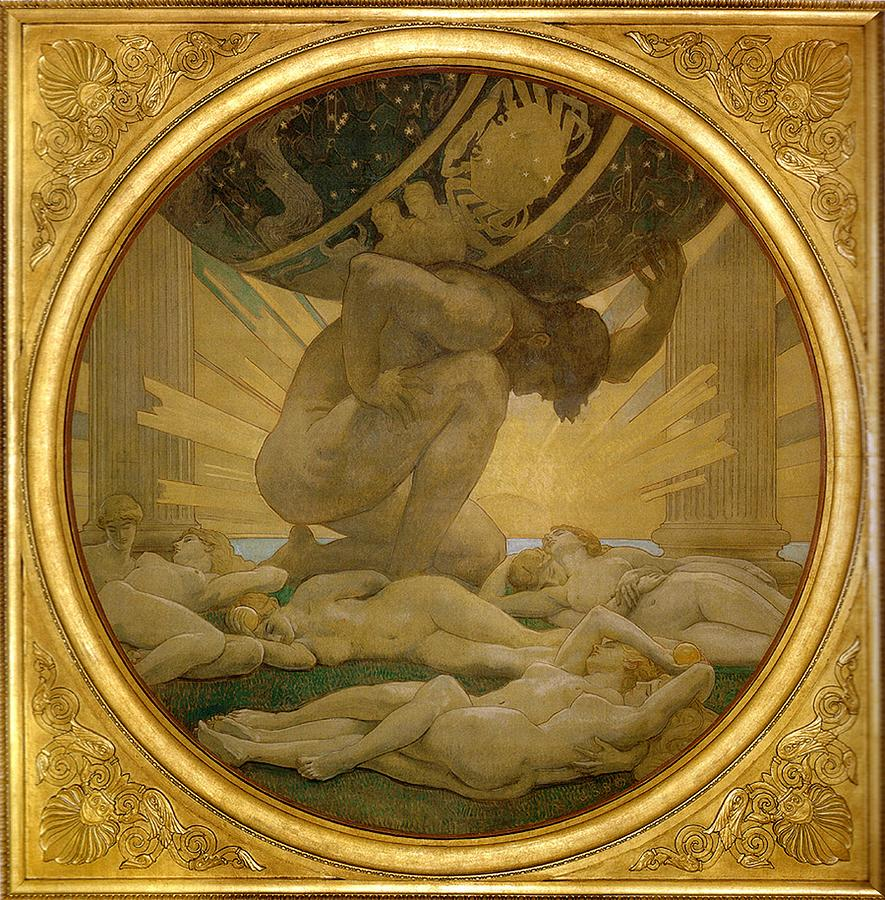
\includegraphics[scale=0.1]{./Images/Atlas.jpeg}
 

\textit{Figure 1: Titan Atlas and the Hesperides, by John Singer Sargent, ca. 1922-1925}
\end{wrapfigure}

King Atlas is said to have invented the celestial sphere, and perhaps even first having established the science of astronomy. He was supposedly skilled in philosophy, mathematics and astronomy. Perhaps this led to his connotation of carrying the firmament. King Atlas inspired cartographer Gerardus Mercator, famous for the Mercator projection of earth, to name his world-maps after him. The Atlantic Ocean was named after Atlas the titan, as well.  

In his late dialogue Timaeus, the philosopher Plato refers to King Atlas as being the first ruler of Atlantis, a city established by Poseidon. Perhaps this city might have referred to a place which is now known as the Richat Structure, a geological formation of concentric circles in northern Mauritania just below the Atlas Mountains, matching the description given by Plato. During the purported existence of this city, 12.000 years ago during the African humid period, this area was a lush and fertile land, until the sudden catastrophic global warming event known as the Younger Drias took place, turning the area into the Sahara Desert we know today. Neolithic artefacts from this era have been found around the Richat Structure, as well as fluvial and torrential deposits from the time the Younger Drias is believed to have taken place. Perhaps this was the origin of the myth of its sudden destruction, having been passed on through oral tradition of North African peoples, until it reached the Egyptian priest Sonchis, who Plato claims to be the source of the story. 

We have chosen to name our language after Atlas because of his legendary reputation as being the ruler of a Utopian civilisation, a symbol of knowledge, as well as his connotation with philosophy and organised knowledge about the world. It seems appropriate to us to name our language Atlan, being somewhat of an encyclopaedic philosophical language, after this ancient cross-cultural figure representing wisdom and the bridge between heaven \nopagebreak and earth. 


\section{Need for an IAL -- {\small Jonathan Roose}}
Historically the diversity of languages has been both a blessing and a curse. On the one hand has the variety of tongs been a database of ways to understand the world and human expression, on the other it has also led to barriers and in- and outgroups. This is why five of my co-students and I have taken up the ambitious task of creating a so-called International Auxiliary Language (IAL for short), a language that will allow its users to bridge language barriers and lead to mutual understanding between speakers with different mother tongues, a neutral ground on which all international communication can occur. 

The lingua franca’s of today's world that are used in international relations, like French, English or Swahili give hierarchical importance to the language of one particular group and/or state, these languages are bas on political power and historical conditions, they cannot be neutral, they have become international languages because of political interactions and thus are always a political matter. The aim of an IAL is to be a meeting ground of all people without it being dependent on power relations and historical animosities. This project has a lot in common with others IALs, Esperanto, for example, made by L.L Zamenhof with the hope that a collective language will lessen the violence between nations. However, why Esperanto succeeded is also why it is limited. It was made to bring speakers of European languages together and it did, for a small part, however, only speakers of European languages. Such languages are commonly referred to as ‘Euroclones’. Our goal with this project is to create a unifying international language for the whole world, which can thus not be limited to only a small set of language groups. 

The ambition we have with the language Atlan is to create a language that is based on nothing more that the human condition. Later in this book Stijn will explain more how we intend to do this however, for now I would like to introduce a term that might help to better understand what we hope to achieve with Atlan. A {\it tertium comparationis} is a wish of many translators to have some way to compare the meaning of the original text with their translation. Deriving from the Latin for ‘a third comparison’ this term describes the want for a ‘perfect language’ that could be used to completely translate a given text. Of course, the translation is meant to have the same meaning however, some meaning will always get lost, the comparison is to see whether the new meaning has not lost the essence of the original. Whether the very quiddity of the original meaning is captured in the translation. What translators want is a semiotic system that can show the essence of a message in a way that can be compared to all other languages. In Atlan we hope that we can create a linguistic code, the rules of grammar and use of a language, that can function as such a {\it tertium comparationis} by making it based on the essential human experiences. A language that can get to the essence of a thing by basing it on the basic human ontological being. This language will function as an IAL that is neutral and universal, it is a language based on the human condition that every human experiences. 


\section{Eco's words -- {\small Jonathan Roose}}


\noindent In this ambitious project we are indebted to the numerous projects that predate ours with the same or similar aims. Not only is there Zamenhof’s Esperanto many more thinkers have dealt with the quest for an IAL. To name all would be too numerous however we can mention a book that has introduced many of the language projects to us. Umberto Eco’s book \textit{The Search for the Perfect Language} has been a great source of inspiration in this project. Like Esperanto the book is mostly concerned with Europe. Nonetheless to finish this introduction to Atlan we end with a passage from his book to summarise the project: 

\begin{quote}
\begin{singlespace}
“Is it possible to reconcile the need for a common language and the need to defend linguistic heritages? Both of these needs reflect the same theoretical contradictions as well as the same practical possibilities. The limits of any international common language are the same as those of the natural languages on which these languages are modelled: all presuppose a principle of translatability. If a universal common language claims for itself the capacity to re-express a text written in any other language, it necessarily presumes that, despite the individual genius of any language, and despite the fact that each language constitutes its own rigid and unique way of seeing, organizing and interpreting the world, it is still always possible to translate from one language to another. However, if this is a prerequisite inherent to any universal language, it is at the same time a prerequisite inherent to any natural language. It is possible to translate from a natural language into a universal and artificial one for the same reasons that justify and guarantee the translation from a natural language into another. The intuition that the problem of translation itself presupposed a perfect language is already present in Walter Benjamin: since it is impossible to reproduce all the linguistic meaning of the source language into a target language, one is forced to place one’s faith in the convergence of all languages. In each language ‘taken as a whole, there is a self-identical thing that is meant, a thing which, nevertheless, is accessible to none of these languages taken individually, but only to that totality of all of their intentions taken as reciprocal and complementary, a totality that we call Pure Language [reine Sprache]’” (Eco 1995:345)
\end{singlespace}
\end{quote}

\section{Linguistic relativity -- {\small Max Geraerdts}}

To start I would like to explore linguistic relativity. It is an important term within the study of linguistics, and I would like to explore the possible consequences it has for a universal language. For those of you who are unfamiliar with this term, it refers to the hypothesis that Sapir and Whorf – two linguists – developed about how the structure of a language can influence our thinking. Sapir and Whorf developed two hypotheses about this presumed phenomenon. A strong and weak hypothesis, the strong one argues that language determines thought and that linguistic categories limit and determine cognitive categories. Effectively stating that the language one speaks limits their cognitive abilities. This hypothesis is now disregarded by many modern linguists. The weak hypothesis, however, is still a main point of discussion among linguists. It argues that language influences thought but does not determine it. This weaker version is much easier to accept. A good example of this is the way in which different languages have different perceptions of colors, representations of time and other elements of cognition. So, while it is safe to say that the strong hypothesis is false it is difficult to deny that language does have an influence on our way of thinking. Language is our way of representing the world. A difference in language can lead to a difference in our representation of the world. 

 
	Ideas and views that would eventually go on to become to define linguistic relativity are first found in ancient philosophy. However, it only began to enter mainstream research in the eighteenth and nineteenth century, with German romantic philosophers on the forefront. (German) nationalism fuelled the discussion about language and its relationship with culture and unity at this time. Wilhelm von Humboldt – a Prussian philosopher, linguist and government functionary – stated in 1820:  

\begin{quote}
\begin{singlespace}
The diversity of languages is not a diversity of signs and sounds but a diversity of views of the world (Traband, 2000). 
\end{singlespace}
\end{quote}

After this movement in Europe, American scientists began discussing this same subject in the early twentieth century. At this time the idea that some languages were superior to others was commonly accepted. It was thought that lesser languages maintained their speakers in intellectual poverty (Migge, 2007). This caused some American linguists to seek to eradicate Native American languages, they thought that its speakers were savages and needed to speak English to become civilized. The first linguist that began refusing these beliefs was the American Franz Boas, during his studies he became fascinated with the Inuit. After learning their language and culture he began stressing the equal worth of all cultures and languages. There were no such thing as lesser languages according to Boas. Boas’ student Edward Sapir went back to the Humboldtian idea that language is vital to understand the unique perception everyone has of our world (Leavitt, 2010). Sapir argued that no two languages could never be perfectly translated to each other. This dissonance in language continued in the world view of individuals according to Sapir: 

\begin{quote}
\begin{singlespace}
	No two languages are ever sufficiently similar to be considered as representing the same social reality. The worlds in which different societies live are distinct worlds, not merely the same world with different labels attached (Sapir, 1929).
\end{singlespace}
\end{quote}

This did not however mean that Sapir agreed with the strong hypothesis, he did in fact disagree with it. Stating that: 

\begin{quote}
\begin{singlespace}
	It would be naïve to imagine that any analysis of experience is dependent on pattern expressed in language (Sapir, 1946).
\end{singlespace}
\end{quote}

So, it seems that in these middle stages of the development of linguistic relativism views on the subject changed dramatically over the years. As we continue through history, we arrive at the linguist Benjamin Lee Whorf. Whorf was one of Sapir’ students and has been associated with linguistic relativity more than any other linguist. One of his best-known examples regards the different words the Inuit have for snow compared to the one word we have for it in English. This example showed that you could not perfectly translate even simple concepts such as snow between languages. This example was however later contested as a misinterpretation by Whorf (Pullum, 1991). Another example of Whorf’s linguistic relativity was the time in Hopi. Whorf argued that the Hopi did not have countable units of time compared to the SEA – standard European languages – the Hopi instead regarded time as a single continuous concept. This notion was however also later contested by other linguists. In the 1980’s Ekkehart Malotki claimed that he had not found any evidence for the claims Whorf had made about the Hopi. This refute was then in its turn contested by relativist scholars who criticized Malotki’s study for forcing the Hopi language into a grammatical model that didn’t fit the data (Lee, 1996). How Whorf approached the Hopi is an example of the structure-centered approach. This approach focuses on a structural difference between languages. It then examines the possible consequences and ramifications of this structural difference. The Hopi and the peculiar structure time has in their languages is a prime example of this approach (Lucy, 1997).  Whorf died at 44 and left many unpublished papers, these were eventually published in a single volume titled \textit{Language, Thought and Reality.} Since neither Sapir nor Whorf had officially formulated a hypothesis Brown and Lenneberg – two influential linguists from the twentieth century – formulated their own in 1954:  

\begin{quote}
\begin{singlespace}
(i) "The world is differently experienced and conceived in different linguistic communities" and (ii) "Language causes a particular cognitive structure" (Brown, 1954).
\end{singlespace}
\end{quote}

These were later reformulated by Brown into the \textit{weak} and \textit{strong} formulations: 

\begin{quote}
\begin{singlespace}
{Structural differences between language systems will, in general, be paralleled by non-linguistic cognitive differences, of an unspecified sort, in the native speakers of the language.} (Weak) 

{The structure of anyone's native language strongly influences or fully determines the worldview he will acquire as he learns the language. (Strong)} 

\end{singlespace}

\end{quote}

Thus, we have arrived at the creation of the Sapir-Whorf hypothesis. Which was not created by Sapir or Whorf. What we have also seen is the difficulty of quantifying linguistic relativity. We have seen many bold claims which have all in turn been contested by others. With this reflection we arrive at the last stretch of the development of linguistic relativity. In 1996 the anthology \textit{Rethinking Linguistic Relativity} was published. It discussed linguistic relativity that focuses more on cognition and social aspects of language. For example, men speaking Guugu Yimithirr could give directions based on a compass-like system of north, south, west and east (Levinson, 1998). This shift of focus alongside the development of better means of conducting research ushered in much new research seeking to not only define but quantify linguistic relativity.  

 
	Brown and Lenneberg thought that languages described the same objective reality. They decided to research if the difference in describing this reality could be proven to have influence on behaviour. For their experiments they decided to focus on the different descriptions of colour in different languages. For one of their first experiments, they tested whether it was easier for English speakers to remember colour shades for which there existed a specific word opposed to shades which were more difficult to describe with words. Later they also compared results between English and Zuni speakers – Zuni classifies green and blue as the same – and it was found that Zuni speakers did have more difficulty making distinctions between shades in the green/blue category (D’Andrade, 1995). These studies by Brown and Lenneberg began a tradition of investigating linguistic relativity through colour terminology. Real differences could be seen between the perception of colour by an individual and the language they speak. These studies however also received criticism because colour perception is hardwired into the brain. This causes it to be universally restricted by some factors for all humans (Lucy, 1997). I however have some nuance to add to this argument. While it is true that colour perception is hardwired into our neural system, I believe linguistic relativity to be a quale. A relativity regarding our experiences, thoughts and inner dialogue. While it is undoubtedly true that colour perceptions are \textit{biologically} the same for all of us, I believe the real difference lies in our \textit{mental} representation of this biological phenomenon.  

 
	Colour research was continued by Berlin and Kay, an anthropologist and linguist respectively who are most well known for their research in colour. During their research they found clear universal conventions when it comes to colour naming. For example, they found that although different languages have different colour terminology, there are universal trends among them. Languages who only have three colour terms all have the same three colours, black, white and red (Berlin, 1969). Because colour naming was originally thought to be random, this new information was seen as a powerful argument against linguistic relativity (Grumperz, 1996). This criticism has since in turn been criticised by relativists such as Lucy who argued that the conclusions from Berlin and Kay were skewed because they insisted that colour terms only encoded colour. According to Lucy, this made them blind to instances were colour terms contained and provided other information that might be considered as linguistic relativity (Lucy, 1992). As we see and discuss more aspects of linguistic relativity it should become clear that it is a very broad and contested hypothesis.  

 
	Advances in cognitive psychology and cognitive linguistics again brought a new wave of studies that focused on linguistic relativity. George Lakoff, for example argued that language is often used metaphorically and that this metaphorical use can give us insight in the cognitive effect of language. He gave the example that in the English language time is often likened with money, a lot of metaphors including time talk about it like it can be invested, saved and spent. This cognitive relationship submerging through language can be a sign of linguistic relativity. Especially considering that other languages do not talk about time this way. Other metaphors like this that are based on human experience are languages where up is associated with good and down with bad. This association can be seen in many myths and folklore, such as heaven being high up in the skies and hell being down. Lakoff also argued that metaphors play an important role in political debates such as the “right to life” or “right to choose” (Lakoff, 1980). Lakoff revitalized linguistic relativity not only because of his newly found results, but also because he reappraised linguistic relativity thus rendering past criticisms moot. He did this by concluding that the debate regarding linguistic relativity had been confused. To clear up this confusion Lakoff described four parameters on which researchers differed in their opinions on what constitutes as linguistic relativity. These were his four parameters: 

\begin{quote}
\begin{singlespace}

\noindent 1. The degree and depth of linguistic relativity. Perhaps a few examples of superficial differences in language and associated behavior are enough to demonstrate the existence of linguistic relativity. Alternatively, perhaps only deep differences that permeate the linguistic and cultural system suffice. 

    \noindent 2. Whether conceptual systems are absolute or whether they can evolve 

    \noindent 3. Whether the similarity criterion is translatability or the use of linguistic expressions 

    \noindent 4. Whether the focus of linguistic relativity is on language or in the brain (Lakoff, 1987)

\end{singlespace}
\end{quote}

\noindent Lakoff concluded based on these definitions that past critics of linguistic relativity had based their criticism on novel definitions of linguistic relativity. According to him this rendered their criticism superficial. 

 
	Up to this point we have mostly seen the broad general way linguistic relativity has developed through history. In this last part I want to focus more on some specific cases and thoughts I have about linguistic relativity. Beginning with its influence on constructed languages and literature. Because there are many instances where authors have used language – natural or constructed – in their stories. One of the best examples of this is how George Orwell showed how linguistic relativity might be exploited for political purposes. The authoritarian state in his novel 1984 created a language Newspeak which made it impossible for people to criticize them (just like Atlan, Newspeak also has some Olig synthetic features: see chapter 5.1.1). Another example is Rand’s \textit{Anthem}, a story about a dystopian communist society who erased the word “I” from their language to erase individuality. Ideas like this illustrate not only the possibility of language on us but also the fact that we can think about language in this way. The fact that we can imagine it having such an influence on ourselves speaks volumes. 

  
	Looking back in history we can see the influence language has had on us and our actions. Book burning illustrates this perfectly. The earliest occurrence dates back to 600 BC. Maybe most famous example coming from the 1930’s and 40’s when the Nazi’s burned countless Jewish books. The Nazi’s sought to erase Jewish culture and saw burning their books which were written in their language about their culture to be necessary. While terrible, it does illustrate that language is inseparable from culture. Seeking to eradicate one demands eradicating the other. Which in turn means that creating one requires creating the other. Linguist and author J.R.R. Tolkien did exactly this when writing stories set in Arda, the most famous of those being \textit{The Lord Of The Rings and The Hobbit.} 

 
	Others sought to create a language to enable a higher level of cognition. They believe that by speaking a new – better – language humans can reach higher levels of thought. One of these languages is Loglan and its evolution Lojban. This conlang is extremely logic based. They seek to be as logical as possible. The creators wanted to use it to test whether linguistic relativity exists. Because the language is entirely based on logic, they thought that it would make its speakers think more logically. Speakers of Lojban reported that they did feel like they thought more logically when speaking Lojban (Nicholas, 2003). Another example of how language can influence our thoughts in a specifically directed way. Another linguist who sought to do this using her Conlang is Suzette Haden Elgin. She has invented the language Láadan which according to its creator makes it easier to express a female world view. Elgin argued that SEA languages have a male centered world view. Using linguistic relativity, she sought to counter this using language. The Toki Pona language was created with the same intent. Its creator – Sonja Lang – wanted to create a simple universal language which focused on happy thoughts. It quite literally aims to make its speakers happier (Lang, Sonja). Because of its simple nature (having only 123 words total), however, it cannot be used to express more detailed or complex meaning: its word for ‘complicated’ is even the same as the word for ‘bad’, \textit{‘ike’.} We once again see that language can have a directed influence on our thoughts. It is not a stretch to pose that we are all confined by our language. It is our way of expressing our thoughts, desires and feelings. The following quote by Von Humboldt illustrates this beautifully: 

\begin{quote}
\begin{singlespace}
“…there resides in every language a characteristic worldview . . . By the same act whereby [man] spins language out of himself, he spins himself into it, and every language draws about the people that possesses it a circle whence it is possible to exit only by stepping over at once into the circle of another one (Von Humboldt, 1988).”
\end{singlespace}
\end{quote}

\noindent Throughout this chapter we have seen the evolution and creation of linguistic relativity. We have seen that it is a difficult topic to pin down and reach consensus on. We have, however, also seen that it does have a remarkable effect on our thinking and understanding of the world. All the way from colours to how we feel. We have seen that we can create languages to infuse its speakers with a certain world view. The power of language is evidently not to be underestimated and we can only guess at the future. Will there be one universal language one hundred years from now? Is one universal language desirable? One way or another, language has and always will be an integral part of our being. For without it we are left soulless.  

\noindent {\it Language \& culture} 

\noindent Language and culture have long been inseparable. They influence each other and evolve alongside each other. Culture needs language and language needs culture. Learning a new language has made this painfully obvious to me. At one point you figure out that it is not sufficient to just learn the meaning of a word according to the dictionary. To then use grammar to construct sentences. Language is more intricate; words can mean one thing in each context only for another context to change its meaning to the complete opposite. Some words are not even in the dictionary. Some words have an entirely different meaning than the one stated in the dictionary. The meaning of some words changes dramatically over time. Some might even say that depending on which language we speak our view of the world can change. Not only this but language grows over time, it is never in a stable state. As is our world and culture.  

We can see clearly that culture influences our language. When culture changes our language changes with it. A good example of this is Dutch ‘straattaal’- literal translation; street language – an unofficial dialect spoken by the youth subculture in the Netherlands. ‘Straattaal’ consists of mostly normal Dutch words and sentence structure, it has however a few exceptions. It introduces new words and ignores grammar in certain situations. Hereby marking itself different from standard Dutch and dominant Dutch society. This diversion is not an accident. These youths don’t want to be a part of mainstream or ‘adult’ society. They seek to define themselves, creating their own language plays a big role in this. It creates a very strong in-group – people who speak the language and can communicate with each other – and a very distinct out-group – people who do not speak the language – this helps in creating subcultures. The fact that a lot of subcultures have their own variations of the language of the dominant culture marks the importance of language in society and the bilateral relation between language and culture.  

This makes it difficult to imagine a language without any culture attached to it. This is, however, one of the goals we have with Atlan. We want to create a language that is as universal as possible. We cannot have one dominant culture associated with Atlan as this would result in a bias for people from that culture. In this chapter I want to explore by what we really mean when we say universal language and what our vision is of the culture that could be attached to Atlan in the future. Because a language without any culture is impossible.  

\noindent \textit{Culture } 

\noindent As you have read in the introduction our goal with Atlan is to create a universal auxiliary language. Not based on one country, culture or region but based on human experiences. I however believe – as implied in the introduction – that a language is impossible to exist without an attached culture. I view language as I do the chicken and egg dilemma. It is impossible for one to exist without the other also existing. This conclusion seems like a problem for Atlan. Our goal is to create a universal language but at the same time it is impossible for a language to be without culture. And therefore, it is also impossible for a language to be without biases. I, however, believe to have found two possible solutions to this problem. The first option is to accept that Atlan has no culture and therefore is not a proper language. This might seem like a shocking conclusion, and I will elaborate on it later. The second option is to attempt to create a new culture attached to Atlan. A culture based on human experiences.  

\noindent \textit{Language without culture} 

\noindent The first option I want to discuss is the language without culture option. Seeing how I have stated earlier that I believe a language without culture is impossible you might be confused by this option. Let me explain what it precisely is I mean when I say language without culture. This option originates from the dilemma of making a universal language. For this to be true it cannot depend on a culture. If it did it would not be universal anymore. But it is also true that without a culture Atlan cannot be a language. I will not go into detail on the precise conditions something has to satisfy to be a language, but I will conclude that having an associated culture is one of them. A result then of the decision to not have any culture associated with Atlan is that Atlan is not a language. Now of course it will still satisfy a lot of the conditions of being a language. It can be spoken and written, and its main purpose is to communicate with other people. But it will not be a language like we know them. It will not have a culture. It will not have a country where it is the official language of. It will not have a history. It will in some sense be more like a computer language. It will not naturally evolve over time it will instead receive updates when deemed necessary.  

This might feel like it makes Atlan a very cold and empty thing. Which it does. I think, however, that for the purpose we devised for this language this is a necessary sacrifice. Atlan will be a universal language, used for communication between people who speak different languages. Atlan does not need to be a language as we know it today because it will fulfill a different purpose. It is okay for Atlan to not have its own culture, history, country and people because we already have enough language who have those things. Atlan will be used as a worldwide communication language; it is allowed to be cold and lifeless. For those languages with identity already exist and will continue to exist in the future. The purpose of Atlan will be to bridge the gap between these cultures. It will be cold and cultureless for everyone; this will make it an even playing field for all those who speak it. This would be the main future I see for Atlan without culture.  

\textit{Language with many cultures} 

If you strongly disagree with the idea of language without culture you are lucky because I have a second option, language with many cultures. It is impossible for Atlan to have one culture because it would be biased towards that culture. It would create an ‘in’ and ‘out’ group, a fatal flaw for a supposed universal language. To avoid this problem, we could have many cultures associated with Atlan. This would create many groups who all have their own variation on Atlan. They can understand each other but they will also each have their own identity. This way Atlan can be used to communicate internationally but it will also have an identity, culture and history. In fact, it will have many different ones. This would create the option for different countries/cultures to develop their own version of Atlan with which they will build their own history with. Of course, these variations cannot be too big otherwise these different groups will not be able to understand each other anymore. But apart from this restriction this solution offers a much more alive version of Atlan than the previous one.  

An obvious argument against this option would be one that argues for one universal culture that is associated with Atlan. This seems like the perfect solution. Atlan will have an associated culture and it will be a universal one. Thus, not excluding anyone and maintaining its purpose as a universal language. I don’t think this is possible unfortunately. Creating one universal culture is a worthy ideal but I am afraid it is not yet possible. As I have said before a culture creates ‘in’ and ‘out’ groups. I believe that culture not only creates these groups it needs them. It originates from them. We can see throughout history that a common enemy brings people closer together. This is also the case for culture. The effect of trying to create a universal group with everyone is impossible. There needs to be some sort of ‘out’ group. The effect of this choice would be very similar to the language with many cultures' choice. There would be many variations in Atlan, all of them associated with their own culture. It is best to have this view from the very beginning of Atlas´ journey, giving the speakers this freedom rather than having them take it.  

I see these as the two possible solutions for the problem I stated in the introduction. It remains a fact that a universal language cannot have a culture. It would not be universal anymore. Having a language without a culture would mean it will not be a language anymore. This poses a problem. I offer two possible solutions for this problem. The first one is to create a language without a culture. The second solution is to create a language with many cultures. These solutions are extremes on the same spectrum. I don’t know which of these solutions is the best solution. I do think that they both solve the problem albeit in their own way. They would have massively different consequences for Atlan in the future. I look forward to seeing how Atlan will develop in our society in the future.
